\documentclass[a4paper, 12pt]{article}
\usepackage[top=3cm, bottom=3cm, left=2.5cm, right=2.5cm]{geometry}
\usepackage[german]{babel}
\usepackage{hyperref} % For clickable links
\usepackage{lmodern}  % Improved font rendering
\usepackage{setspace} % Adjust line spacing
\usepackage{graphicx} % For better layout options
\usepackage{titlesec} % For custom section formatting

% Title Formatting
\titleformat{\section}{\large\bfseries\centering}{\thesection}{1em}{}
\titleformat{\subsection}{\normalsize\bfseries}{\thesubsection}{1em}{}

% Custom Title
\title{\vspace{-1cm}SWEN1 - Intermediate Protokoll}
\author{
    \textbf{Samuel Hammerschmidt} \\
    \href{https://github.com/shammerschmidt1999/SWEN1}{\texttt{GitHub: github.com/shammerschmidt1999/SWEN1}}
}
\date{November 2024}

\begin{document}

\maketitle

\section{Einführung}
\subsection{Projektstruktur}
Das Projekt ist in mehrere Klassen aufgeteilt. Durch Vererbung und Polymorphismus wird eine einfache Erweiterung des Spiels ermöglicht. Die Klassen sind in verschiedene Dateien aufgeteilt, um die Struktur des Projekts übersichtlich zu halten. Die Klassen sind in verschiedene Namespaces aufgeteilt, um eine klare Struktur zu gewährleisten. Die Klassen sind in verschiedene Namespaces aufgeteilt, um eine klare Struktur zu gewährleisten. Die Klassen sind in verschiedene Namespaces aufgeteilt, um eine klare Struktur zu gewährleisten.
Die Klassen sind in verschiedene Namespaces aufgeteilt, um eine klare Struktur zu garantieren.
Weiters wurden Interfaces implementiert, um die Klassen flexibler und austauschbarer zu machen.
Klassen haben neben ihren Properties auch private Fields, dies dient der Steuerung des Zugriffs auf die Eigenschaften.
Die Verwendung von Enumerationen verbessert die Lesbarkeit des Codes und ermöglicht eine einfache Erweiterung des Spiels.
Der integrierte HTTP-Server ermöglicht die Benutzerregistrierung und -anmeldung. Benutzer werden derzeit noch nicht in einer Datenbank gespeichert, sondern nur im Arbeitsspeicher. Die Implementierung der Datenbankanbindung ist für das Final Hand-In geplant.

\subsection{Anforderungen für Intermediate Hand-In}
Für die Zwischenabgabe stehen vor allem die Klassen \texttt{User} und \texttt{Card} sowie die für den HTTP-Server benötigten Klassen im Fokus. Diese werden im Laufe des Protokolls genauer beschrieben. Weitere technische Entscheidungen werden ebenfalls erklärt.

\vspace{0.5cm}
\section{Klassenbeschreibung}
\subsection{User}
Die \texttt{User}-Klasse repräsentiert einen Benutzer des Spiels. Sie enthält die folgenden Attribute:
\begin{itemize}
    \item \texttt{static Dictionary<string, User> \_Users}: Eine Liste von Benutzern, die im Spiel registriert sind.
    \item \texttt{string Username}: Der Benutzername des Spielers.
    \item \texttt{string Password}: Das Passwort des Spielers.
    \item \texttt{int Elo}: Die Elo-Zahl des Spielers.
    \item \texttt{Stack UserCards}: Eine Liste von Karten, die der Spieler besitzt.
    \item \texttt{Stack UserDeck}: Eine Liste von Karten, die der Spieler in seinem Deck hat (Untermenge von \texttt{UserCards}).
    \item \texttt{Stack UserHand}: Eine Liste von Karten, die der Spieler in der Hand hält (Untermenge von \texttt{UserDeck}).
    \item \texttt{Stack UserDiscard}: Eine Liste von Karten, die der Spieler abgeworfen hat (Untermenge von \texttt{UserDeck}).
\end{itemize}

Die \texttt{User}-Klasse enthält die folgenden Methoden:
\begin{itemize}
    \item \texttt{void PrintUser()}: Gibt die Informationen des Spielers auf der Konsole aus.
    \item \texttt{void PrintStack(Stack stack)}: Gibt die Informationen einer Kartenliste auf der Konsole aus.
    \item \texttt{static void Create(string username, string password)}: Erstellt einen neuen Benutzer und fügt ihn zur Liste der registrierten Benutzer hinzu.
    \item \texttt{static (bool Success, string Token) Logon(string username, string password)}: Loggt den Benutzer ein und gibt ein Token zurück, falls die Anmeldedaten korrekt sind.
    \item \texttt{void Save(string token)}: Ändert die Informationen des Benutzers und speichert diese.
    \item \texttt{static User? Get(string userName)}: Gibt den Benutzer mit dem gegebenen Benutzernamen zurück.
    \item \texttt{static bool Exists(string userName)}: Überprüft, ob ein Benutzer mit dem gegebenen Benutzernamen existiert.
\end{itemize}

Ein User wird über den integrierten HTTP-Server erstellt und eingeloggt.

\subsection{Card}
Die \texttt{Card}-Klasse repräsentiert eine Karte im Spiel. Sie enthält die folgenden Attribute:
\begin{itemize}
    \item \texttt{string Name}: Der Name der Karte.
    \item \texttt{double Damage}: Dier Schaden, den die Karte verursacht.
    \item \texttt{ElementType ElementType}: Der Elementtyp der Karte.
\end{itemize}

Die \texttt{Card}-Klasse enthält die folgenden Methoden:
\begin{itemize}
    \item \texttt{abstract void PrintInformation()}: Abstrakte Methode, die die Informationen der Karte auf der Konsole ausgibt.
\end{itemize}

Die \texttt{Card}-Klasse ist eine abstrakte Klasse, von der die Klassen \texttt{MonsterCard} und \texttt{SpellCard} erben.
\subsection{MonsterCard}
Die \texttt{MonsterCard}-Klasse repräsentiert eine Monsterkarte im Spiel. Sie erbt von der \texttt{Card}-Klasse und enthält folgende zusätzliche Attribute:
\begin{itemize}
    \item \texttt{MonsterType MonsterType}: Der Monstertyp der Karte.
\end{itemize}
Die \texttt{PrintInformation()}-Methode wird überschrieben, um die Informationen der Monsterkarte auf der Konsole auszugeben.

\subsection{SpellCard}
Die \texttt{SpellCard}-Klasse repräsentiert eine Zauberkarte im Spiel. Sie erbt von der \texttt{Card}-Klasse und enthält keine zusätzlichen Attribute.
Die \texttt{PrintInformation()}-Methode wird überschrieben, um die Informationen der Zauberkarte auf der Konsole auszugeben.

\subsection{Weitere Klassen}
Es wurden bereits zahlreiche weitere Klassen implementiert, (z.B. Battle, Stack, CoinPurse, etc.) die jedoch nicht im Detail beschrieben werden, da diese für das Intermediate Hand-In nicht relevant sind.

\section{Design- und technische Entscheidungen}
\subsection{GlobalEnums}
Die \texttt{GlobalEnums}-Klasse ist eine statische Klasse, die alle Enumerationen enthält, die im Spiel verwendet werden. Sie enthält die folgenden Enumerationen:
\begin{itemize}
    \item \texttt{ElementType}: Die Elementtypen der Karten (Fire, Water, Normal).
    \item \texttt{MonsterType}: Die Monstertypen der Monsterkarten (Dragon, Goblin, Wizard, Knight, Ork, FireElve, Kraken).
    \item \texttt{CoinType}: Die Münztypen (Diamond, Platinum, Gold, Silver, Bronze).
    \item \texttt{RoundResult}: Die Ergebnisse einer Runde (Victory, Defeat, Draw).
\end{itemize}
Die Verwendung einer globalen Klasse für die Enumerationen ermöglicht eine einfache Anwendung der Enumerationen in verschiedenen Bereichen des Spiels.
Weiters führt die Verwendung von Enumerationen zu einer verbesserten Lesbarkeit des Codes und die globale Sammlung der Enumerationen ermöglicht eine einfache Erweiterung und eine übersichtliche Struktur.

\subsection{HTTP-Server}
Der HTTP-Server wurde implementiert, um die Benutzerregistrierung und -anmeldung zu ermöglichen. Der Server verwendet die \texttt{HttpListener}-Klasse, um HTTP-Anfragen zu empfangen und zu verarbeiten. Der Server enthält die folgenden Endpunkte:
\begin{itemize}
    \item \texttt{POST /user/}: Erstellt einen neuen Benutzer.
    \item \texttt{POST /session/}: Loggt einen Benutzer ein.
\end{itemize}

Der HTTP-Server funktioniert folgendermaßen:
\begin{enumerate}
    \item In der \texttt{Program}-Klasse wird ein \texttt{HttpSvr}-Objekt erstellt und gestartet. Der Server lauscht auf eingehende HTTP-Anfragen.
    \item Das Incoming-Event des Servers wird mit der Methode \texttt{Svr\_Incoming} verknüpft, die aufgerufen wird, wenn eine Anfrage eingeht.
    \item Die Methode \texttt{Svr\_Incoming} empfängt die Anfrage und gibt die HTTP-Methode, den Pfad und die Header der Anfrage auf der Konsole aus.
    \item Basierend auf dem Pfad der Anfrage wird entschieden, welcher \texttt{Handler} die Anfrage weiterverarbeiten soll. Dies geschieht durch die \texttt{HandleEvent}-Methode der {Handler}-Klasse.
    \item Wenn der Pfad \texttt{/users} enthält, wird die Anfrage an den \texttt{UserHandler} weitergeleitet. Wenn der Pfad \texttt{/sessions} enthält, wird die Anfrage an den \texttt{SessionHandler} weitergeleitet. Andernfalls wird eine 404-Fehlermeldung zurückgegeben.
    \item Jeder spezifische \texttt{Handler} erbt von der \texttt{Handler}-Klasse und kann die \texttt{Handle}-Methode überschreiben, um spezifische Logik für die Verarbeitung der Anfrage zu implementieren.
    \item Die \texttt{HttpSvrEventArgs}-Klasse enthält Informationen über die eingehende HTTP-Anfrage, einschließlich Methode, Pfad, Header und Payload.
    \item Die Methode \texttt{Reply} der \texttt{HttpSvrEventArgs}-Klasse wird verwendet, um eine HTTP-Antwort an den Client zu senden, einschließlich Statuscode und optionalem Antworttext.
\end{enumerate}

\subsection{Tokens}
Für die Authentifizierung der Benutzer wird ein Token-System verwendet. Beim Einloggen wird ein Token generiert und an den Client zurückgegeben. Dieses Token wird bei jeder Anfrage des Clients an den Server mitgeschickt und dient zur Authentifizierung des Benutzers. Das Token wird im Arbeitsspeicher gespeichert und ist nur für die Dauer der Sitzung gültig. Das Token wird beim Ausloggen oder nach einer gewissen Zeit ungültig.

\subsection{Interfaces}
Für die meisten Klassen wurden Interfaces implementiert. Dies hat den Grund, dass die Klassen dadurch flexibler und austauschbarer werden. So kann z.B. ein \texttt{MonsterCard}-Objekt als \texttt{Card}-Objekt behandelt werden, wenn es das \texttt{ICard}-Interface implementiert. Dadurch können Methoden, die ein \texttt{Card}-Objekt erwarten, auch ein \texttt{MonsterCard}-Objekt akzeptieren.
Das führt zu einer verbesserten Lesbarkeit und Wartbarkeit des Codes und ermöglicht eine einfachere Erweiterung des Spiels.

\subsection{Fields und Properties}
Für jede \texttt{public} Property wurde ein \texttt{private} Field erstellt, um den Zugriff auf die Eigenschaften zu steuern. Dies ermöglicht eine bessere Kontrolle über den Zugriff auf die Eigenschaften und ermöglicht die Implementierung von Validierungslogik und Berechnungen in den Eigenschaften.

\pagebreak

\section{UML-Diagramme}
\subsection{Klassendiagramm User und Card}
\begin{figure}[h]
    \centering
    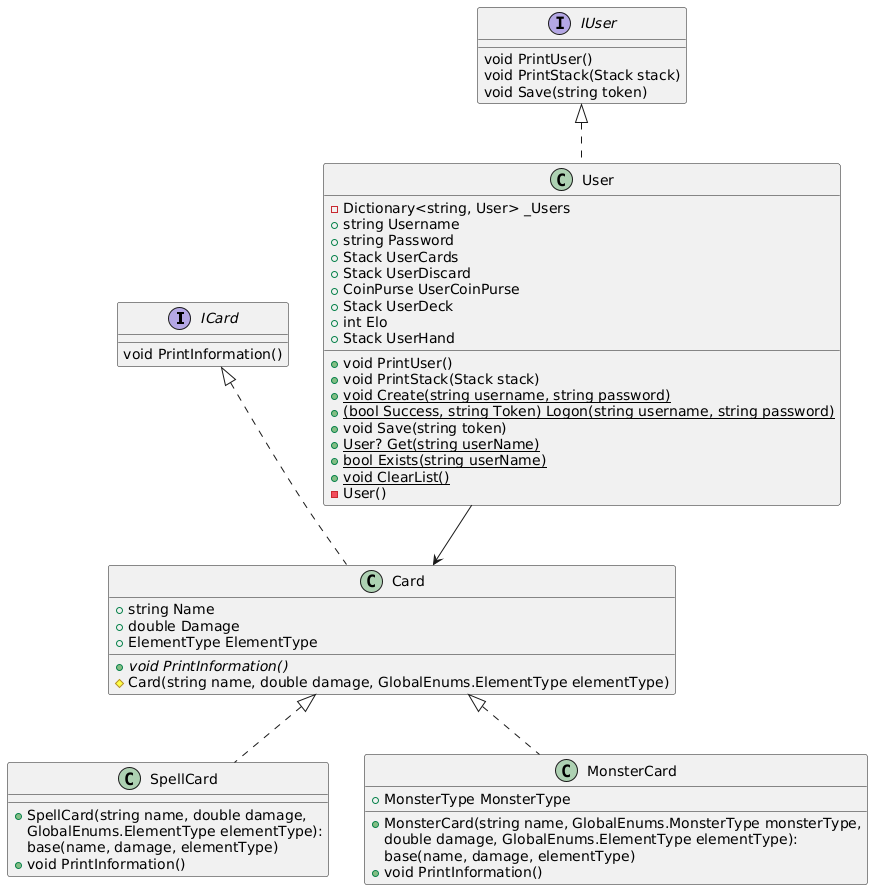
\includegraphics[width=0.8\textwidth]{User_Card_UML.png}
    \caption{Klassendiagramm der Klassen User und Card}
\end{figure}

\begin{figure} [h]
    \centering
    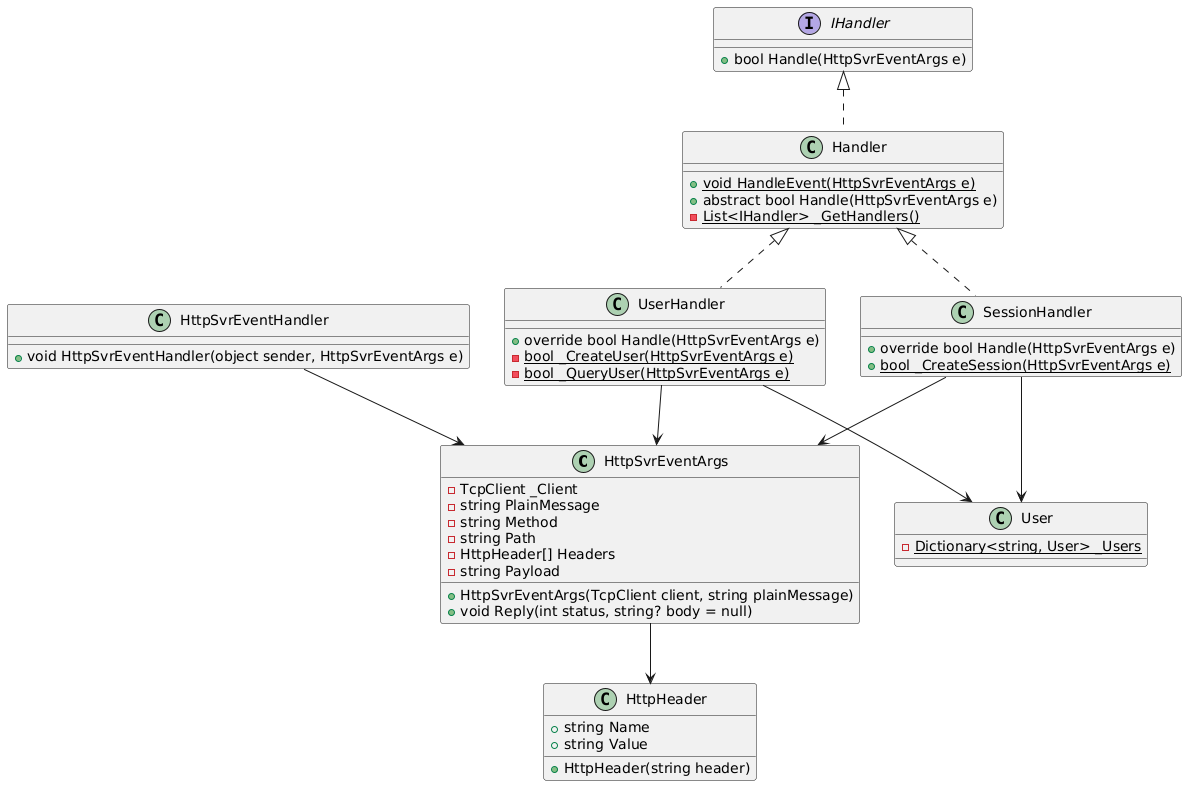
\includegraphics[width=0.8\textwidth]{Handler_HTTP_UML.png}
    \caption{Klassendiagramm der Klassen HTTP-Server und Handler Klassen}
\end{figure}

\end{document}
